\documentclass{article}

\usepackage{graphicx}
\usepackage{tikz}
\usepackage{tikzsymbols}
\usetikzlibrary{calc,patterns,shapes.geometric}
\pagestyle{empty}
\usepackage[margin=0pt]{geometry}
\geometry{papersize={14in,12in}}

\def\centerarc[#1](#2)(#3:#4:#5){\draw[#1] ($(#2)+({#5*cos(#3)},{#5*sin(#3)})$) arc (#3:#4:#5);}

\begin{document}
	\begin{figure}
		\centering
		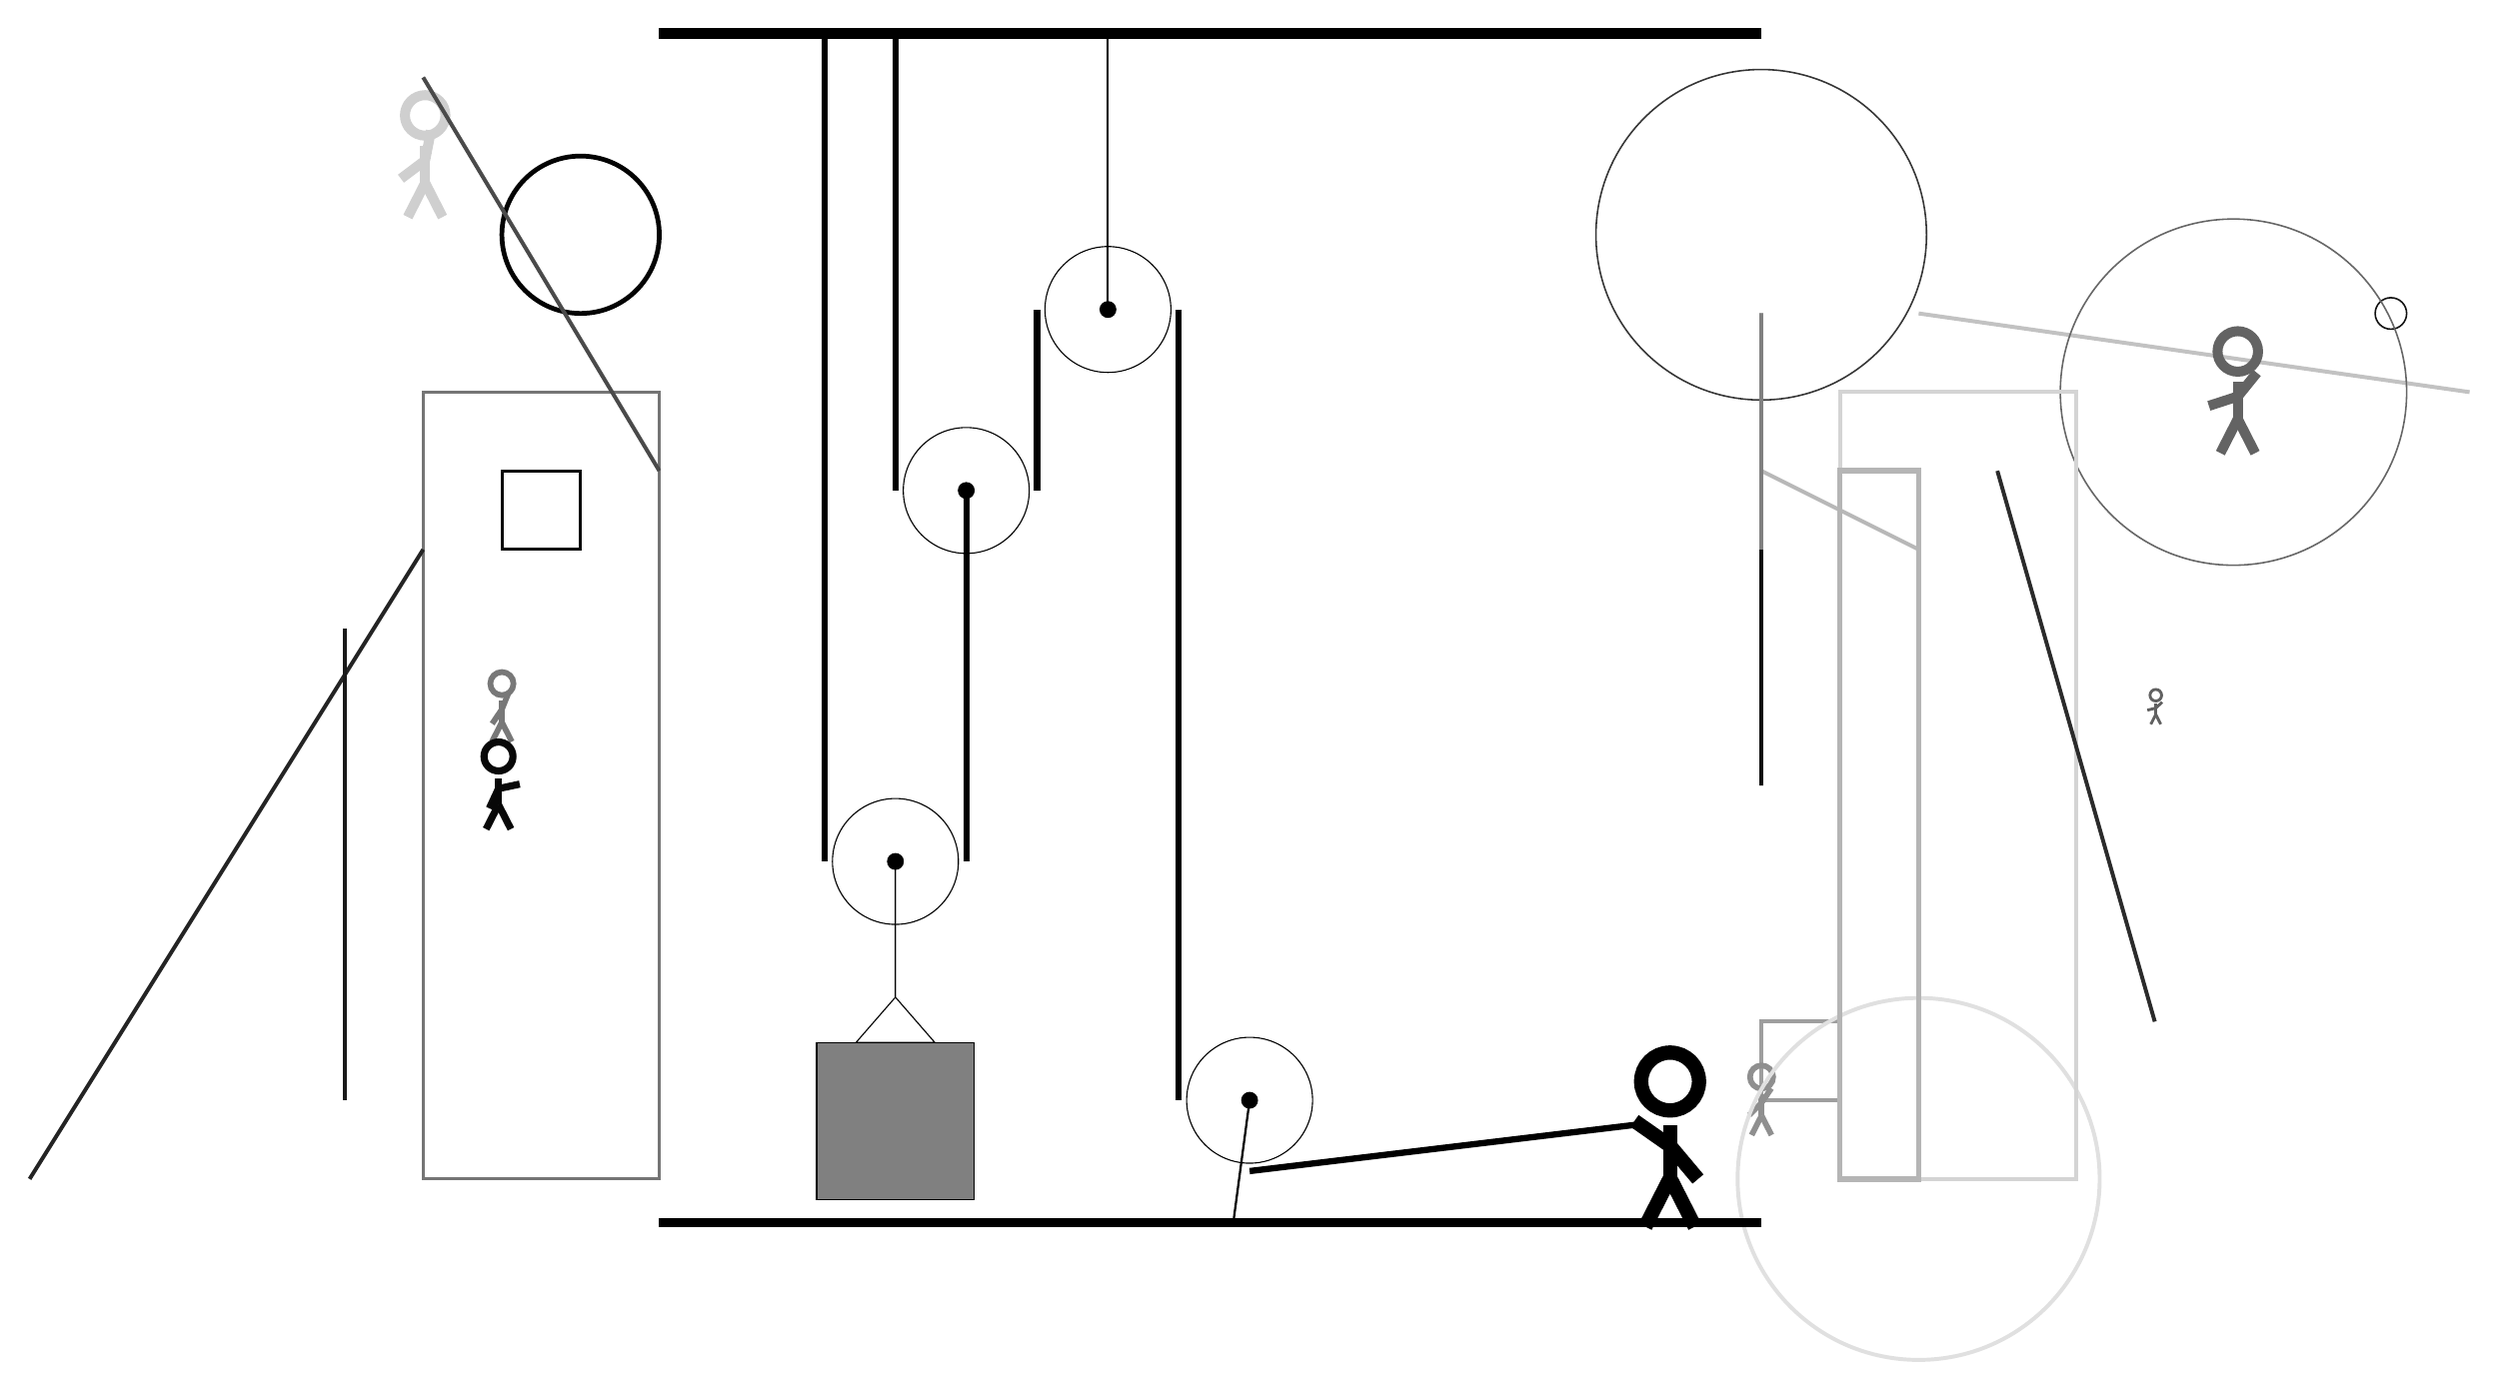
\begin{tikzpicture}
			%%%%% START %%%%%
			
			\draw[fill=black] (-2, 11.5) rectangle (12, 11.625);
			
			\draw (1, 1.035) circle (0.8);
			\draw[fill=black] (1, 1.035) circle (0.1);
			
			\draw (1.9, 5.75) circle (0.8);
			\draw[fill=black] (1.9, 5.75) circle (0.1);
			
			\draw[line width=0.5mm, color=black!24](14, 8) -- (21, 7);
			
			\draw[line width=0.5mm, color=black!28](14, 5) -- (12, 6);
			\draw[line width=0.5mm, color=black!65] (14, -1) rectangle (14, -1);
			\draw[line width=0.5mm, color=black!38] (13, -2) rectangle (12, -1);
			\draw [line width=0.2mm, color=black!79](12, 9) circle (2.1);
			
			\node[line width=0.6mm, color=black!62] at (17, 3) {\Strichmaxerl[2][14][43]};
			
			\draw [line width=0.2mm, color=black!93](20, 8) circle (0.2);
			
			\draw [line width=0.2mm, color=black!60](18, 7) circle (2.2);
			\draw [line width=0.6mm, color=black!99](-3, 9) circle (1.0);
			
			\draw[line width=0.4mm, color=black!54] (-2, -3) rectangle (-5, 7);
			
			\node[line width=0.6mm, color=black!53] at (-4, 3) {\Strichmaxerl[4][56][68]};
			\draw[line width=0.5mm, color=black!86](-5, 5) -- (-10, -3);
			\node[line width=0.5mm, color=black!97] at (-4, 2) {\Strichmaxerl[5][65][12]};
			
			\node[line width=0.4mm, color=black!61] at (18, 7) {\Strichmaxerl[7][18][51]};
			\draw[line width=0.4mm, color=black!95] (12, 8) rectangle (12, 2);
			\node[line width=0.4mm, color=black!44] at (12, -2) {\Strichmaxerl[4][45][56]};
			
			\draw [line width=0.5mm, color=black!12](14, -3) circle (2.3);
			\draw[line width=0.5mm, color=black!17] (13, -3) rectangle (16, 7);
			\draw[line width=0.4mm, color=black!97] (-4, 5) rectangle (-3, 6);
			
			\draw[line width=0.5mm, color=black!50] (12, 5) rectangle (12, 8);
			\draw[line width=0.7mm, color=black!29] (14, -3) rectangle (13, 6);
			
			\node[line width=0.4mm, color=black!19] at (-5, 10) {\Strichmaxerl[7][37][79]};
			\draw[line width=0.5mm, color=black!71](-5, 11) -- (-2, 6);
			\draw[line width=0.5mm, color=black!83](15, 6) -- (17, -1);
			\draw[line width=0.5mm, color=black!90](-6, 4) -- (-6, -2);
			
			\draw (3.7, 8.05) circle (0.8);
			\draw[fill=black] (3.7, 8.05) circle (0.1);
			\draw[thick] (3.7, 8.05) -- (3.7, 11.5);
			
			\draw (5.5, -2) circle (0.8);
			\draw[fill=black] (5.5, -2) circle (0.1);
			\draw[thick] (5.5, -2) -- (5.3, -3.5);
			
			\draw (1, 1.035) -- (1, -0.69) -- (0.5, -1.265) -- (1.5, -1.265) -- (1, -0.69);
			\draw[fill=black!50] (0, -1.265) rectangle (2, -3.265);
			\draw[line width=0.8mm] (0.1, 11.5) -- (0.1, 1.035);
			\centerarc[line width=0.8mm](1, 1.035)(180:360:0.9);
			\draw[line width=0.8mm](1.9, 1.035) -- (1.9, 5.75);
			\draw[line width=0.8mm] (1.0, 11.5) -- (1.0, 5.75);
			\centerarc[line width=0.8mm](1.9, 5.75)(180:360:0.9);
			\draw[line width=0.8mm](2.8, 5.75) -- (2.8, 8.05);
			\centerarc[line width=0.8mm](3.7, 8.05)(0:180:0.9);
			\draw[line width=0.8mm] (4.6, 8.05) -- (4.6, -2);
			\centerarc[line width=0.8mm](5.5, -2)(0:90:-0.9);
			\draw[line width=0.8mm](5.5, -2.9) -- (10.5, -2.3);
			
			\node at (10.8, -2.5) {\Strichmaxerl[10][-35][-50]};
			
			\draw[fill=black] (-2, -3.5) rectangle (12, -3.6);
			
			%%%%% END %%%%%
		\end{tikzpicture}
	\end{figure}	
\end{document}